\documentclass[t, 11pt]{beamer}
\pdfmapfile{+sansmathaccent.map}
%%% Работа с русским языком
\usepackage{cmap}				
\usepackage{mathtext} 				
\usepackage[T2A]{fontenc}		
\usepackage[utf8]{inputenc}			
\usepackage[english,russian]{babel}	

\usetheme{Ilmenau}
\usecolortheme{lily} % Цветовая схема



%%% Работа с картинками
\usepackage{graphicx}

\usepackage{csquotes}

\hypersetup{				
	colorlinks=true,       	
	linkcolor=blue,          
	citecolor=blue,       
	filecolor=magenta,      
	urlcolor=magenta           
}


\title{Word embeddings}
\subtitle{Word2vec Doc2vec}
%\author{Чувакин Сергей}
\date{15.10}
%\institute[<<Анализ больших данных в бизнесе, экономике и обществе>>]{<<Высшая школа экономики>>}
\institute{<<Высшая школа экономики>>}
\begin{document}
	\frame[plain]{\titlepage}
%	\section{Outline}
%	
%	\begin{frame}
%		\frametitle{\insertsection} 
%		\begin{block} {}
%			 
%			\hyperlink{l1}{\beamerbutton{Language models}}
%		\end{block}
%			\begin{block}{}
%		\hyperlink{l2}{\beamerbutton{Probabalistic}}
%		\end{block}
%				\begin{block}{}
%		\hyperlink{l2}{\beamerbutton{Perplexity}}
%		\end{block}
%	\end{frame}
%	

\subsection{Word2vec}
\begin{frame}
	\frametitle{\insertsection}
	\frametitle{\insertsubsection}  
	Word2vec is a combination of models used to represent distributed representations of words in a corpus.
	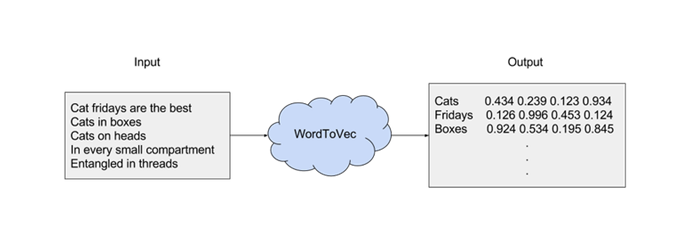
\includegraphics[width=1\linewidth]{word2vec.png} 
\end{frame}


\begin{frame}
	\frametitle{\insertsection}
	\frametitle{\insertsubsection}  
	\begin{itemize}
		\item CBOW
		\item Skipgram
	\end{itemize}
	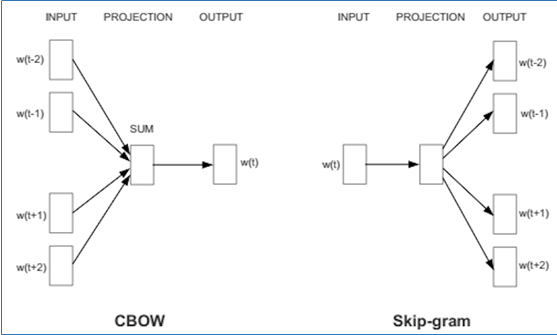
\includegraphics[width=0.8\linewidth]{cbow_skipgram.png} 
\end{frame}


\begin{frame}
	\frametitle{\insertsection}
	\frametitle{\insertsubsection} 
	Example: 
	
	 
	 <<The quick brown fox jumps over the lazy dog.>>
\end{frame}

\begin{frame}
	\frametitle{\insertsection}
	\frametitle{\insertsubsection}  

	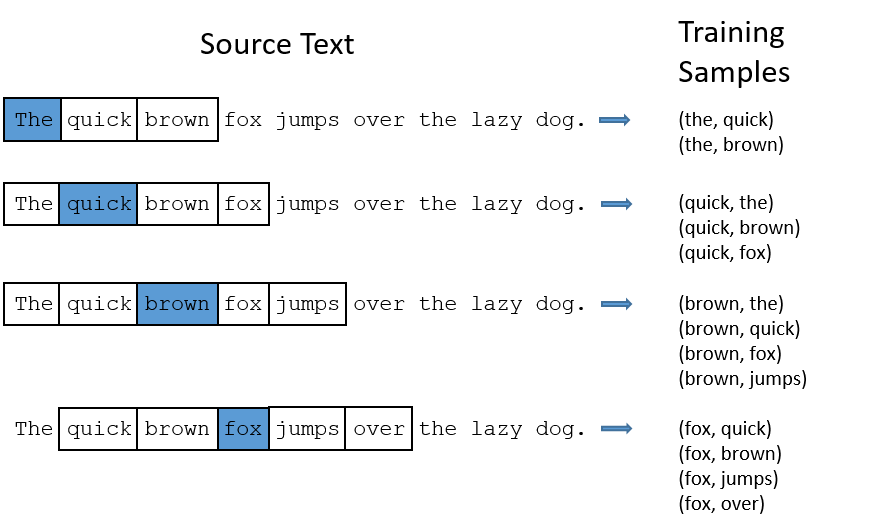
\includegraphics[width=0.8\linewidth]{exam.png} 
\end{frame}



\begin{frame}
	\frametitle{\insertsection}
	\frametitle{\insertsubsection}  
	Architecture.
	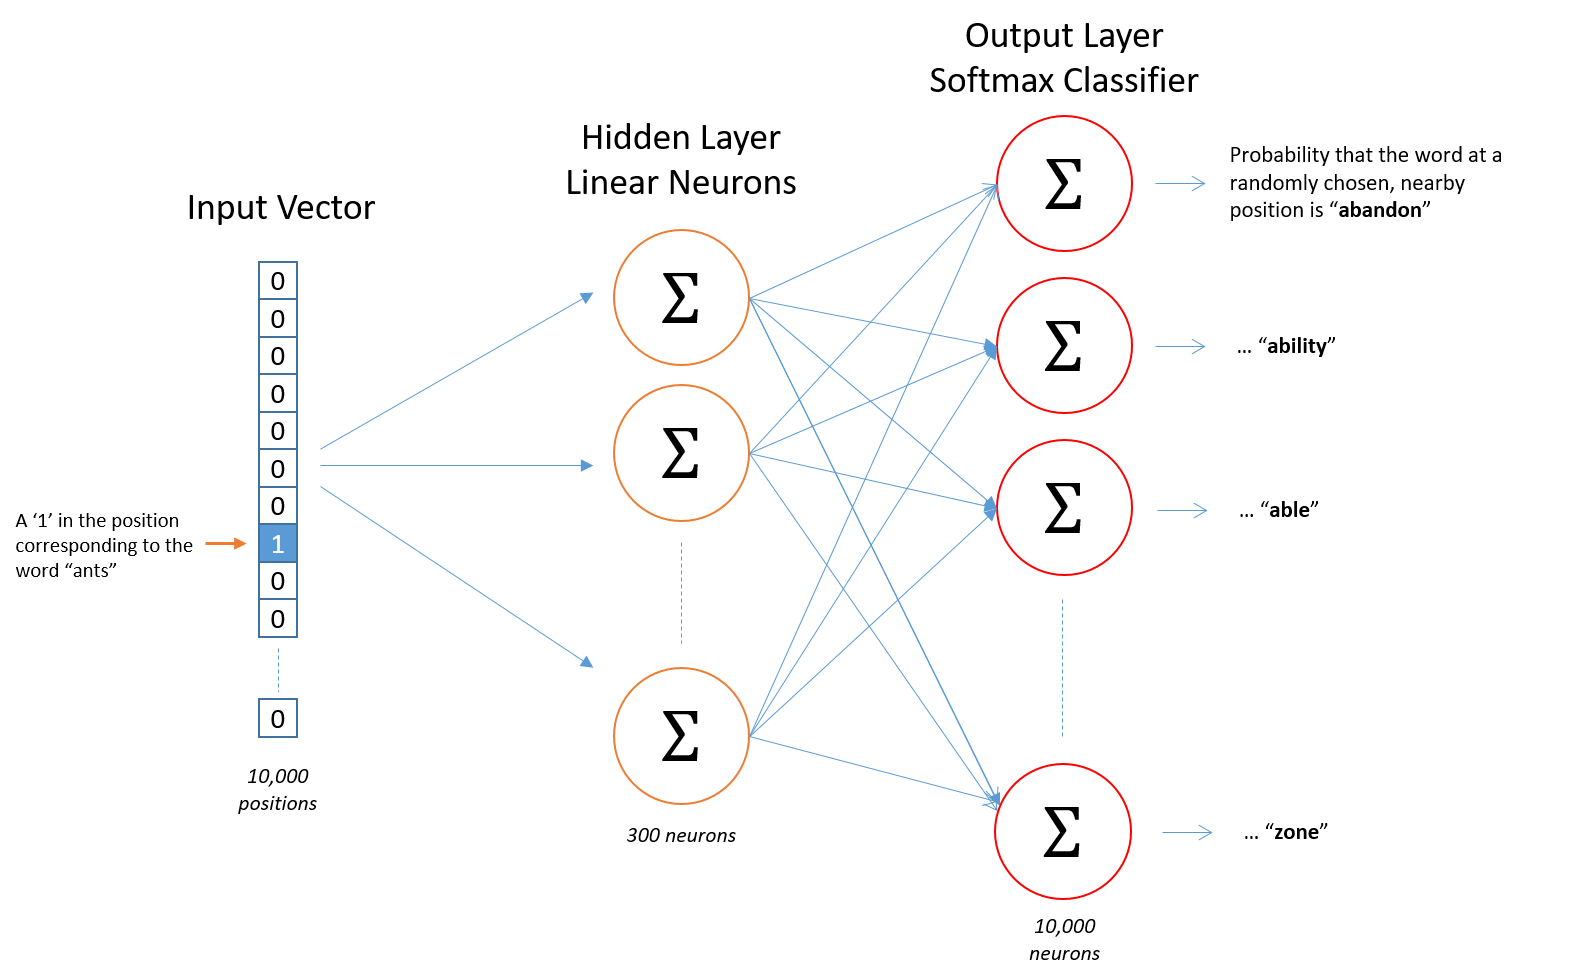
\includegraphics[width=0.8\linewidth]{arch.png} 
\end{frame}

\begin{frame}
	\frametitle{\insertsection}
	\frametitle{\insertsubsection}  
	Output.
	
	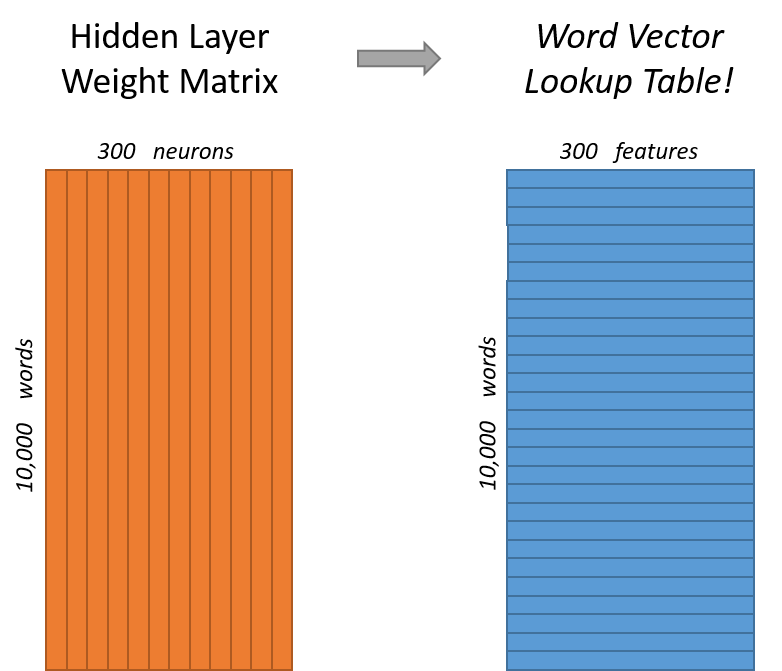
\includegraphics[width=0.6\linewidth]{output.png} 
\end{frame}



\subsection{Doc2vec}
\begin{frame}
	\frametitle{\insertsection}
	\frametitle{\insertsubsection}  
	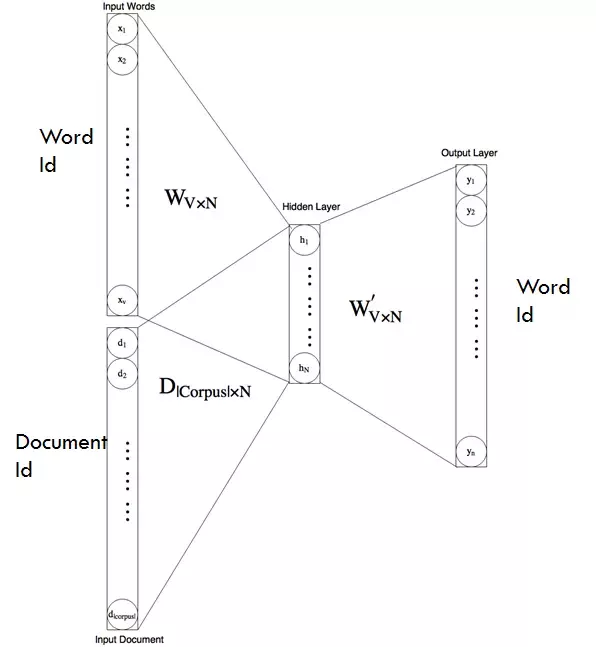
\includegraphics[width=0.6\linewidth]{doc2vec.png} 
\end{frame}









%	\begin{frame}
%	\frametitle{\insertsection}
%	\frametitle{\insertsubsection}  
%	Синонимы кватификаторов 
%	\begin{center}
%		\begin{table}[]
%			\begin{tabular}{c|c|c}
%				\hline
%				Синоним &Расшифровка &Квантификатор \\
%				\hline
%		+ & 1 и более раз &\{1,\}   \\
%		* & 0 и более раз &\{0,\}   \\
%
%		? &  0 или 1 раз& \{0,1\}  \\
%  
%			\end{tabular}
%		\end{table}
%	\end{center}
%\end{frame}

%\begin{frame}
%	\frametitle{\insertsection}
%	\frametitle{\insertsubsection}  
%	Чтобы убрать жаность необходимо добавить ?
%	
%	\vspace{0.5cm}
%	
%	Строка на вход  <<( dfghvb ) sdvsd ( sdcvkjnh ) sdvsd ( dkjhvgr ) sdvfv.>>
%	
%	\vspace{0.5cm}
%	
%	шаблон: r"$\backslash$(.+?$\backslash$)"
%	
%	\vspace{0.5cm}
%	
%	на выходе: ['dfghvb', 'sdcvkjnh', 'dkjhvgr']
%	
%\end{frame}



%	\begin{frame}
%	\frametitle{\insertsection}
%	\frametitle{\insertsubsection}
%	
%	
%	\vspace{1cm}
%	\includegraphics[width=0.9\linewidth]{page2.png}
%	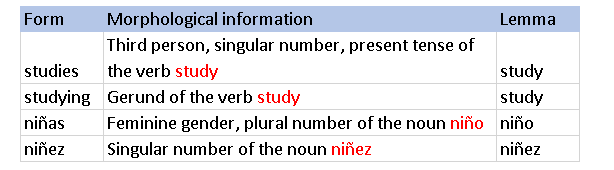
\includegraphics[width=0.7\linewidth]{lem.png}
%\end{frame}
\end{document}